\documentclass[titlepage,a4paper,oneside]{article}
\usepackage[utf8]{inputenc}
\usepackage{amsmath}
\usepackage{mathabx}
\usepackage{graphicx}
\usepackage{minted}
\usepackage{booktabs}
\usepackage[english,spanish,es-noindentfirst,es-nosectiondot,es-nolists,
es-noshorthands,es-lcroman,es-tabla]{babel}
\usepackage{lmodern}             % Use Latin Modern fonts
\usepackage[T1]{fontenc}         % Better output when a diacritic/accent is used
\usepackage[utf8]{inputenc}      % Allows to input accented characters
\usepackage{textcomp}            % Avoid conflicts with siunitx and microtype
\usepackage{microtype}           % Improves justification and typography
\usepackage[svgnames,table,xcdraw]{xcolor}    % Svgnames option loads navy (blue) colour
\usepackage[hidelinks,urlcolor=blue]{hyperref}
\hypersetup{colorlinks=true, allcolors=Navy, pdfstartview={XYZ null null 1}}
\newtheorem{lemma}{Lema}
\usepackage[width=14cm,left=3.5cm,marginparwidth=3cm,marginparsep=0.35cm,
height=21cm,top=3.7cm,headsep=1cm, headheight=1.6cm,footskip=1.2cm]{geometry}
\usepackage{csquotes}
\usepackage{biblatex}
\addbibresource{informe.bib}
\usepackage[pdf]{graphviz}

\graphicspath{ {img/} }


\begin{document}

\begin{titlepage}
\title{
	75.74 \-- Distribuidos I \-- TP4\\
    \large Facultad de Ingeniería\\
	Universidad de Buenos Aires
}
\author{%
  del Mazo, Federico\\
  100029
\and
  Mermet, Ignacio Javier\\
  \texttt{98153}
\and
  Ventura, Julián\\
  \texttt{102391}
}


\date{Junio 2022}

\maketitle

\end{titlepage}

\tableofcontents

\newpage

\section{Sobre la entrega}

El código de la entrega se puede encontrar en \href{https://github.com/CrossNox/7574-TP3}{GitHub}.  Allí se encuentra el \texttt{README.md} que describe la ejecución del código.

\section{Análisis del trabajo a realizar}
El presente trabajo práctico agrega dificultad por sobre la entrega anterior. Si bien la lógica de negocio se mantiene, en esta entrega nos piden diseñar el sistema acorde a un entorno multicomputing y de modo tal que tenga alta disponibilidad.

\subsection{Puntos clave}

\begin{itemize}
\item \textbf{Alta Disponibilidad}: El servidor siempre debe responder a sus clientes, incluso aunque sea un mensaje de que esta ocupado, o que no puede resolver una consulta.
\item \textbf{Tolerancia a fallos}: De cara al cliente, los fallos no deben ser evidentes. El sistema debe poder recuperarse de aquellos fallos que pudieran surgir durante la ejecución del mismo.
\item \textbf{Sincronización}: Los nodos que repliquen su funcionamiento deben sincronizar el estado del sistema.
\item \textbf{Remoción de duplicados}: Ya que no se permite la perdida de mensajes (o mejor dicho, los mensajes perdidos se deben recuperar), en vez de un modelo de \textit{at most once}, se tiene un modelo de \textit{at least once}, por lo que se tiene que contemplar el caso de que a un nodo del sistema le llegue un mensaje duplicado.
\item \textbf{Recuperación de nodos}: El sistema debe garantizar que si un nodo se cae en algún momento de la ejecución esta caída será correctamente identificada, el nodo será re-levantado, y deberá estar nuevamente al día con cualquier evento que haya sucedido en el tiempo intermedio.
\end{itemize}

\section{Hipótesis, simplificaciones y asunciones}

\begin{itemize}
\item El contenedor de RabbitMQ no va a estar replicado ni puede caerse en ningún momento.
\item La sesión entre un servidor y el cliente no puede cortarse.
\item Algunos nodos del sistema podemos considerarlos como un punto singular de fallo, y por ende no replicarlos.
\item Las caídas de nodos son transitorias. Si un nodo muere, eventualmente va a revivir, por lo que se podrá utilizar storage persistente local para almacenar estado.
\item No es un sistema elástico! No van a aparecer nuevos nodos, ni es un caso que tenemos que contemplar. Los nodos caídos son conocidos, configurables en la inicialización.
\item Las ejecuciones de los clientes son secuenciales, el servidor proveerá únicamente una consulta a la vez a los clientes.
\item Los clientes no se caen, por ende no deberán ser tolerantes a fallos.
\item Los clientes cooperan en todo momento con el servidor para llevar a cabo la sesión de forma correcta.
\item Los clientes conocen por configuración una serie de puntos de entrada al servidor, a los que deberán enviar sus consultas.
\item El sistema se encuentra disponible si al menos uno de los puntos de entrada del servidor brinda una respuesta ante una consulta.
\item Los datos enviados por el cliente y confirmados por el servidor no podrán ser perdidos.
\item Una sesión de un cliente con el servidor existirá hasta ser finalizada por el cliente, quién tendrá la obligación de culminarla.
\item El servidor rechazará cualquier inicio de una nueva sesión mientras exista alguna activa.
\end{itemize}

\section{Arquitectura}

\subsection{Nodos de ejecución}

En el siguiente diagrama DAG se puede observar el flujo de datos desde la recepción de los posts y comentarios, hasta la obtención de los resultados finales del cómputo en los nodos marcados como sink.

\begin{figure}[H]
	\centering
	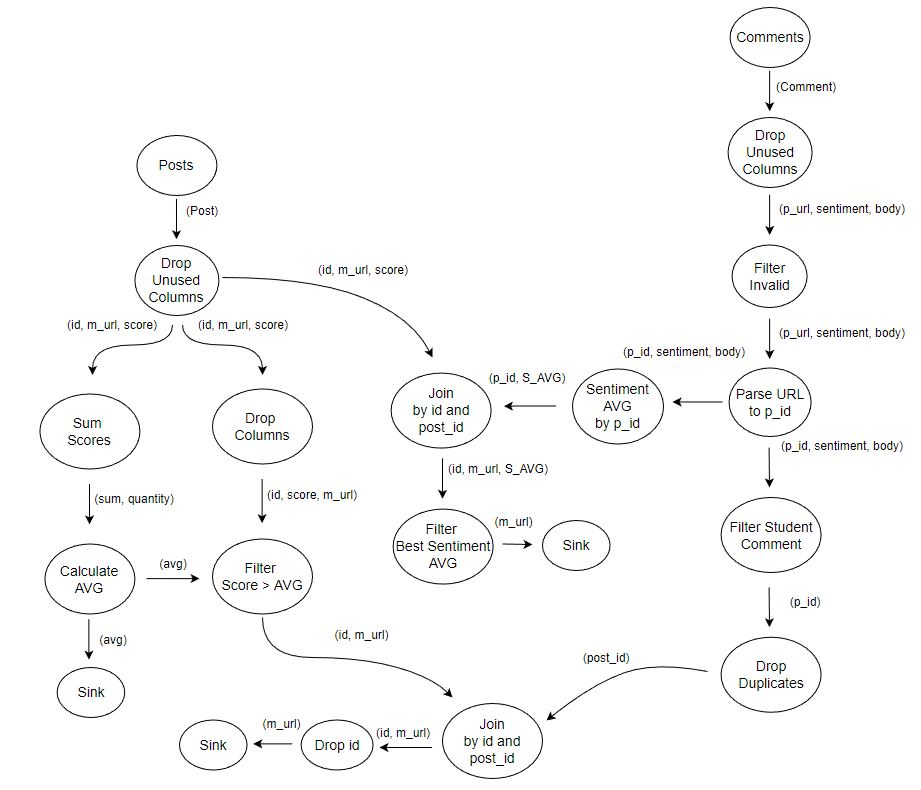
\includegraphics[width=12cm]{img/dag.JPG}
	\caption{Diagrama DAG}
\end{figure}

Las tuplas que acompañan a las aristas representan a los datos que viajan por el pipeline de una etapa a la otra.

Dicho modelo lógico se mapeó a cierto grupo de procesos, los cuales podemos apreciar en los diagramas de robustez.

\begin{figure}[H]
	\centering
	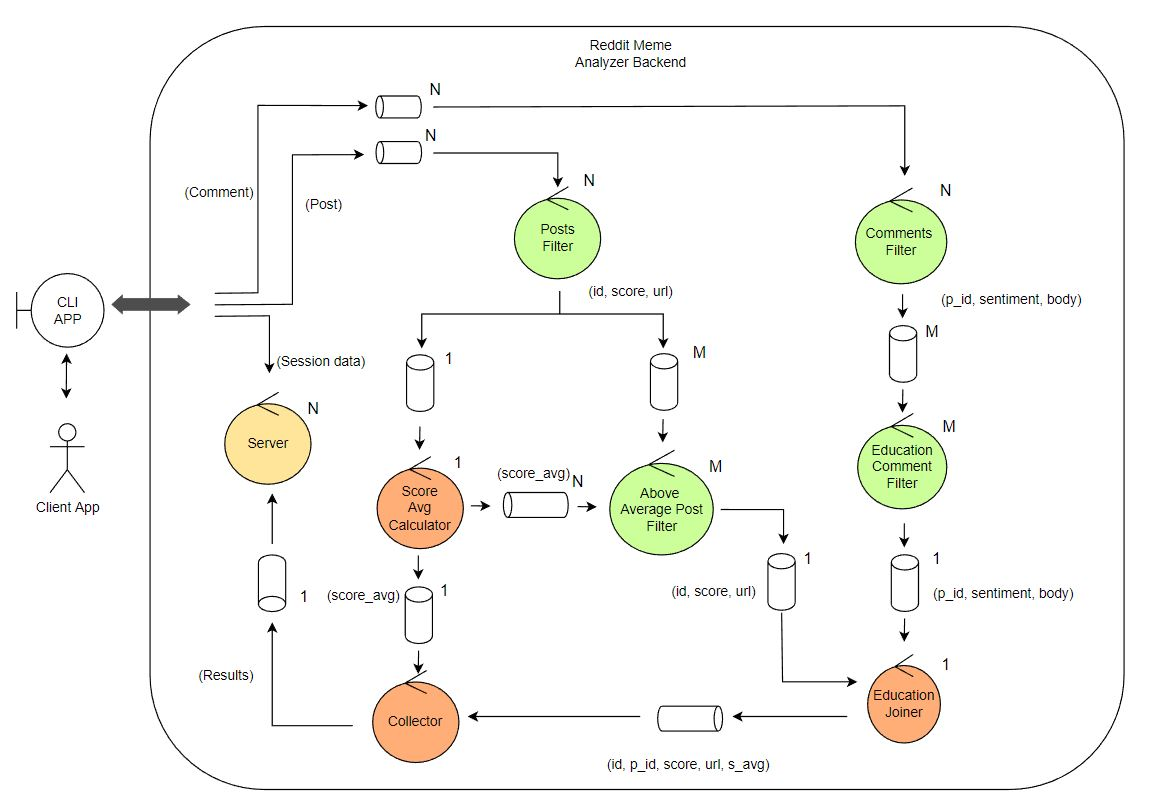
\includegraphics[width=11.5cm]{img/robustez_1.JPG}
	\caption{Diagrama de robustez 1}
\end{figure}


\begin{figure}[H]
	\centering
	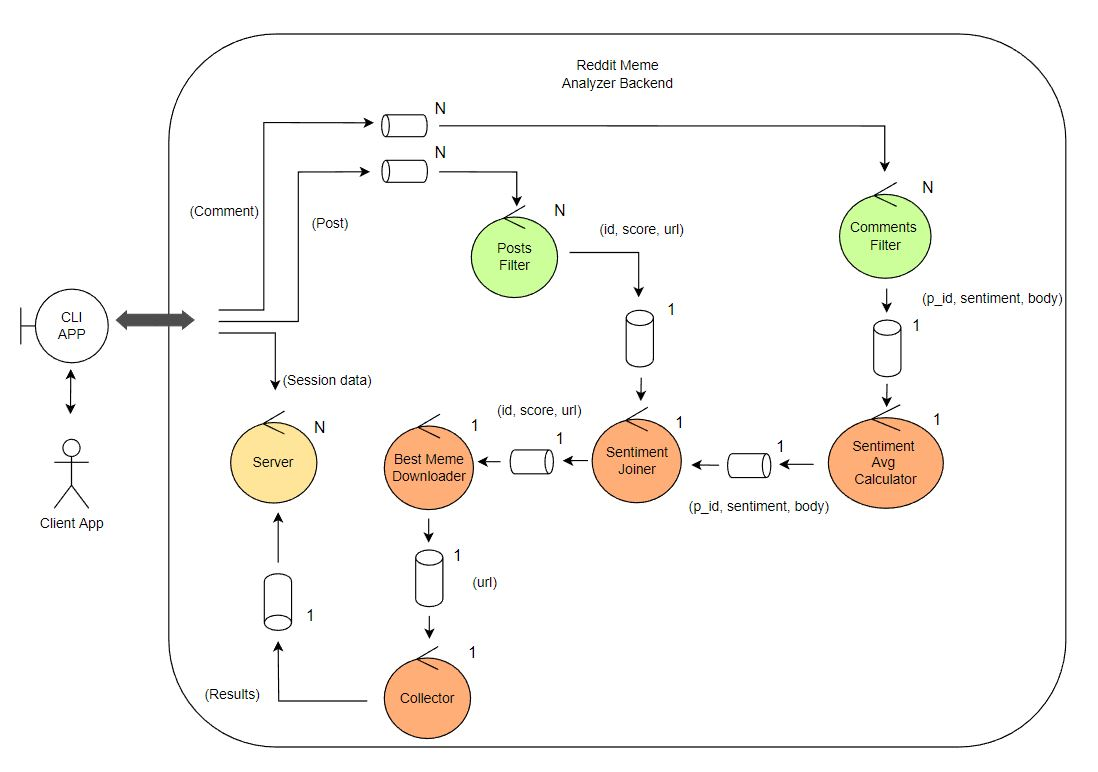
\includegraphics[width=11.5cm]{img/robustez_2.JPG}
	\caption{Diagrama de robustez 2}
\end{figure}

Como puede observarse, los nodos se comunican a través de la utilización de colas, las cuales fueron modeladas con ayuda de un middleware de mensajes basado en RabbitMQ.

En general, cada uno de estos nodos realizará alguna tarea de transformación de mensajes, filtrado de mensajes o \texttt{join} de streams de mensajes.

En líneas generales, un nodo de ejecución aplica el siguiente patrón:

\begin{figure}[H]
\begin{minted}[
    mathescape,
	linenos,
    numbersep=5pt,
    gobble=0,
    frame=lines,
    framesep=2mm]{text}
msg := obtener mensaje de queue de entrada
si msg está en almacenamiento:
    descartar
    enviar ACK a la queue de entrada
    retornar
guardar el mensaje
si el identificador de sesión es inválido:
    descartar
    enviar ACK a la queue de entrada
    retornar
si msg == EOS:
    propagar si es el último EOS
    reset de estado
    enviar ACK a la queue de entrada
    retornar
out := callback(msg)
si out no es nulo:
    enviar out a queue de salida
enviar ACK a la queue de entrada
\end{minted}
\caption{Pseudocódigo de un worker stateless.}
\end{figure}

Algunos nodos son paralelizables y otros no. Aquí hacemos la distinción entre \textcolor{teal}{\textit{nodos stateless}} y \textcolor{orange}{\textit{nodos stateful}}. A lo que hacemos referencia en verdad es a una serie de propiedades correlacionadas:

\begin{enumerate}
    \item Los nodos stateless usan un callback de procesamiento de mensajes que es stateless. Los nodos stateful usan callbacks que son stateful y solo pueden dar resultados al terminar la ejecución.
    \item Los nodos stateless compiten por extraer mensajes de la queue de entrada.
    \item Dado que los callbacks stateful requieren todo el stream de datos, no pueden estar replicados. Los nodos stateless pueden estar replicados.
    \item Las replicas de nodos stateless no se comunican entre sí en ningún momento. No propagan su estado entre sí. La repartición de mensajes entre workers se hace a través del MOM.
\end{enumerate}

En verdad, todos los nodos mantienen un estado a través de la API de almacenamiento, detallada en \ref{APIStorage}.

Si el nodo tuvo un fallo entre que se procesa el mensaje y se deposita el resultado en una queue de salida, el mensaje es re-encolado (ya que nunca se recibió el ACK), haciendo que algún otro nodo del mismo tipo (incluso si mismo) se encargue de manejarlo en el futuro, y así no perder datos. Como desventaja, este diseño nos da una posible duplicidad de mensajes recibidos, los cuales tendrán que ser removidos del sistema. De este modo, podemos garantizar que los mensajes se procesan al menos una vez, dado que el ACK solo se hace al final, y una sola vez, dado que detectamos los duplicados para evitar re-procesarlos.

El siguiente diagrama de clases muestra la abstracción generada para modelizar un nodo del DAG.

\begin{figure}[H]
	\centering
	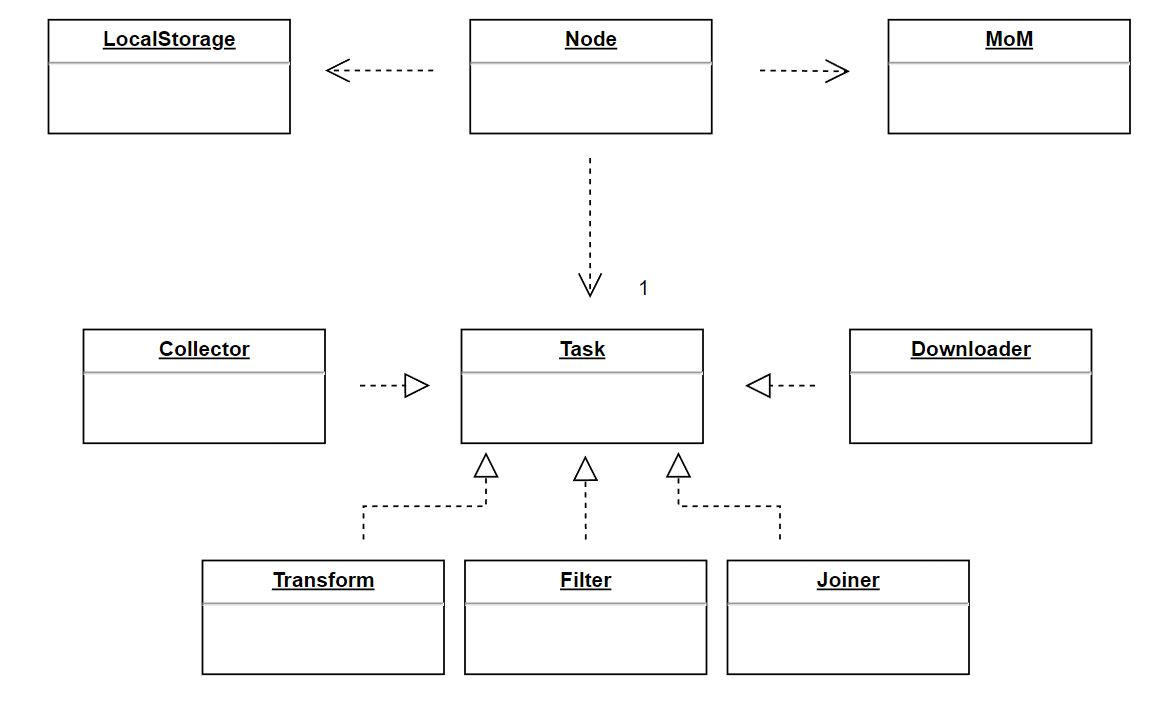
\includegraphics[width=14cm]{img/dag_node_class.JPG}
	\caption{Diagrama de clases para un nodo}
\end{figure}

\subsection{Middleware de Comunicación}

Cómo ya se mencionó, estos nodos se comunican a través de un middleware construido por sobre RabbitMQ.
Este middleware de mensajes busca simplificar la comunicación entre los procesos a partir de dos patrones de comunicación, como son el patrón Ventilator y Publisher Subscriber.

Para esto se mantuvo el concepto de Queue y Exchange que provee RabbitMQ, desembocando en la siguientes abstracciones.

\begin{figure}[H]
	\centering
	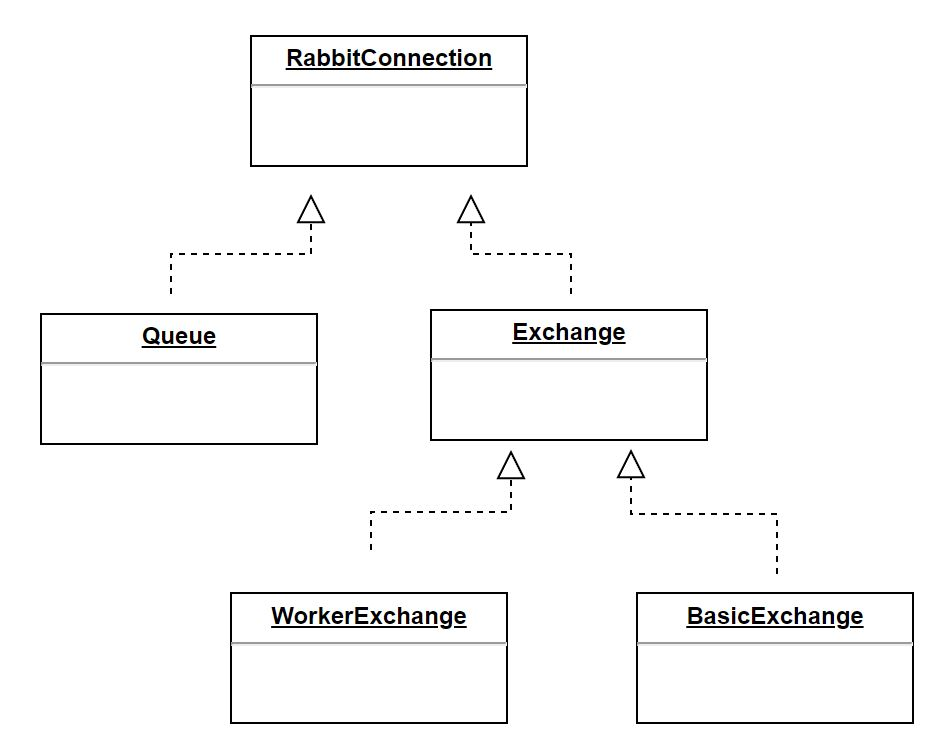
\includegraphics[width=13cm]{img/mom_class.JPG}
	\caption{Diagrama de clases para el MOM}
\end{figure}

En este caso, una Queue es generada por un proceso cuando desea consumir mensajes, abstraído de la necesidad de realizar una conexión con RabbitMQ y la declaración y bindeo de dicha cola a un exchange.

Por otro lado, un proceso productor deberá crear un nuevo Exchange sobre el cuál podrá enviar mensajes.

\begin{itemize}
    \item \textbf{BasicExchange}: Provee una conexión simple entre un productor y un consumidor, utilizando el exchange por default de Rabbit.
    \item \textbf{WorkerExchange}: Provee una conexión que permite declarar a múltiples tipos de consumidores, en base a dos categorías.
        \begin{itemize}
            \item Worker: Este tipo de consumidores compiten por los mensajes entregados al Exchange.
            \item Subscriber: Este tipo de consumidores reciben todos los mensajes entregados al Exchange.
        \end{itemize}
\end{itemize}

Dicha idea fue posible a través de la utilización de un exchange por tópico de RabbitMQ, como se ve en el siguiente diagrama.

\begin{figure}[H]
	\centering
	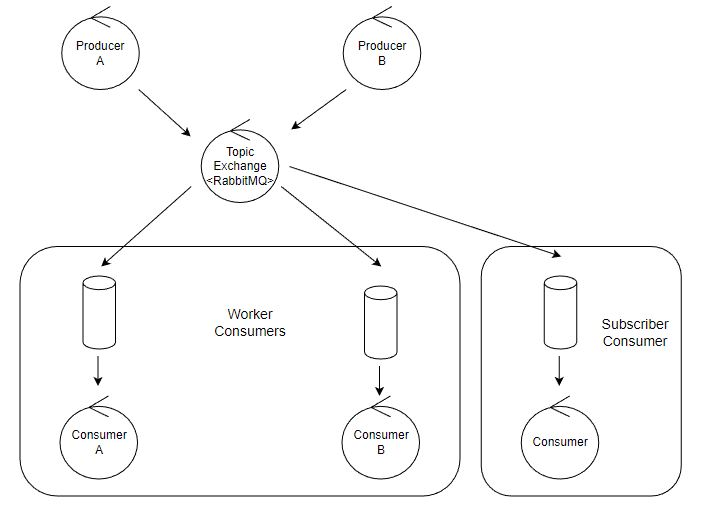
\includegraphics[width=13cm]{img/mom_diagram.JPG}
	\caption{Implementación de MOM a través de RabbitMQ}
\end{figure}

Por cada consumidor existirá una cola exclusiva a él que será unida al exchange de tópico de Rabbit a través de un tópico particular. La idea es que la abstracción de WorkerExchange reparte los mensajes entre 0 y M colas de consumidores en forma Round-Robin, a partir de un tópico asociado al identificador de cada consumidor. Por otro lado, los consumidores tipo Subscriber unirán sus colas escuchando de todos los tópicos, posibilitando así que se obtengan todos los mensajes.

Entonces, cada WorkerExchange generado por un productor deberá realizar las siguientes tareas.
\begin{enumerate}
    \item Declarar un exchange por tópico de RabbitMQ bajo un nombre solicitado.
    \item Declarar M colas, correspondientes a los M consumidores tipo Worker y bindear cada una a un identificador autoincremental de 0 a M.
    \item Declarar K colas, correspondientes a los K consumidores tipo subscriber y bindear cada una de ellas a todos los tópicos.
    \item Adicionalmente, bindear cada cola declarada a un tópico \texttt{broadcast}, que permite la posibilidad de propagar un mensaje a todos los consumidores.
\end{enumerate}

Dado que implementar el patrón de productor-consumidor de esta forma en la cual cada consumidor escucha de una cola exclusiva a él en lugar de una cola compartida para todos ellos puede traer una perdida de performance, se realizó el siguiente experimento para confirmar si el overhead introducido no es tan grande como para justificar este encare.

\begin{table}[H]
\centering
\begin{tabular}{l|llll|}
\cline{2-5}
\cellcolor[HTML]{FFFFFF}                  & \multicolumn{3}{l|}{\textbf{Topic Exchange}} & \textbf{Workers} \\ \hline
\multicolumn{1}{|l|}{prefetch} & \multicolumn{1}{l|}{\textbf{0}} & \multicolumn{1}{l|}{\textbf{1}} & \multicolumn{1}{l|}{\textbf{1000}} & \textbf{1} \\ \hline
\multicolumn{1}{|l|}{\textit{producer}}   & 5.513               & 5.676      & 5.635      & \textbf{5.343}   \\
\multicolumn{1}{|l|}{\textit{consumer 0}} & \textbf{3.536}      & 6.860      & 4.266      & 8.796            \\
\multicolumn{1}{|l|}{\textit{consumer 1}} & \textbf{2.353}      & 6.834      & 3.210      & 7.239            \\
\multicolumn{1}{|l|}{\textit{consumer 2}} & \textbf{2.112}      & 6.762      & 2.484      & 4.275            \\ \hline
\end{tabular}
\caption{Experimento para comparar las dos alternativas de implementación. En todas las ejecuciones se mandaron $50000$ mensajes, sin prints ni sleeps. Las queues fueron inicializadas como durables.}
\label{exp-dex-wrk}
\end{table}

Como puede observarse, no se aprecia un overhead en la implementación frente a la alternativa común.

\subsection{Servidor de cara al cliente}\label{ServerClient}

La interfaz del sistema al cliente es provista a través del nodo servidor. Este nodo tendrá como tarea proveer una API al cliente que le permita iniciar una sesión, introducir datos en el sistema y obtener los resultados del cómputo.

\begin{figure}[H]
	\centering
	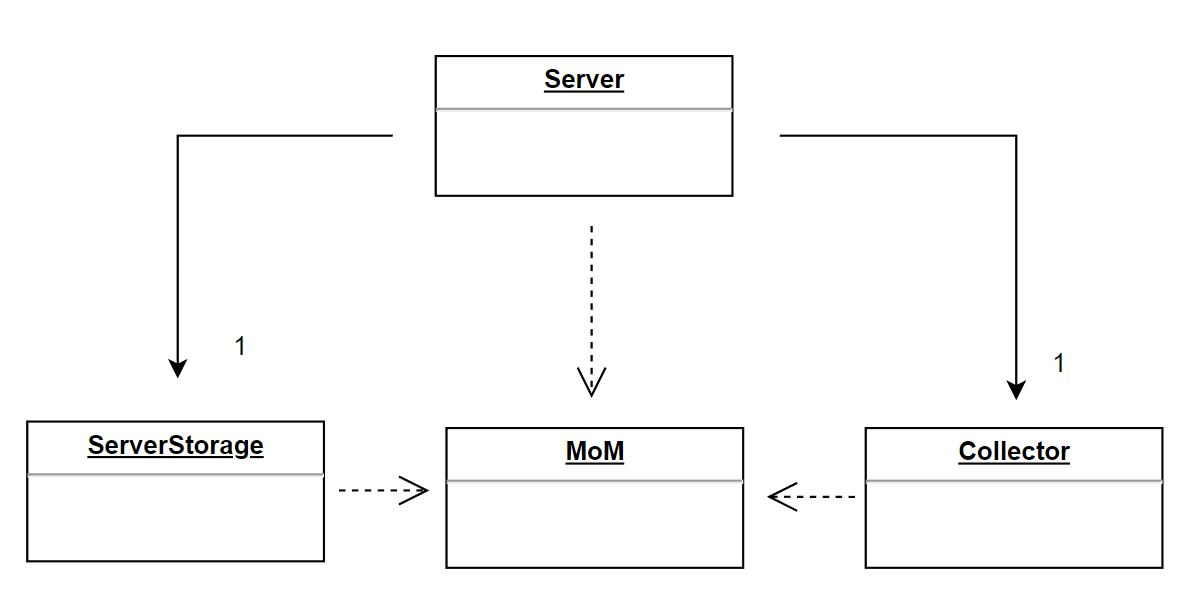
\includegraphics[width=10cm]{img/server_class.JPG}
	\caption{Diagrama de clases para el server}
\end{figure}

La clase Collector provee al servidor de los resultados de la ejecución actual mientras que la clase ServerStorage provee un almacenamiento persistente y distribuido para el mismo. Ambas clases dependen de el Middleware de mensajes antes mencionado para implementar su funcionalidad.

\paragraph{Protocolo de Comunicación}

La comunicación entre el cliente y el servidor se realiza siguiendo un protocolo diseñado en base a las hipótesis antes mencionadas.

Este protocolo puede ser dividido en dos secciones, siendo la primera el manejo de una sesión y la segunda la carga de datos. Para cada una de ellas se utilizó una biblioteca de comunicación distinta.

\begin{itemize}
    \item \textbf{ZMQ}: Para la comunicación del cliente con un nodo servidor, negociando una nueva sesión, solicitando los resultados y finalizando la misma.
    \item \textbf{RabbitMQ}: Para el envío del stream de datos de posts y comentarios, haciendo uso de las garantías de tolerancia a fallos que proveen las colas persistentes.

\end{itemize}

A continuación se muestra un diagrama de secuencia que busca detallar cómo es el flujo de mensajes entre el cliente y el servidor a lo largo de la vida de una sesión, en un escenario sin errores.

\begin{figure}[H]
	\centering
	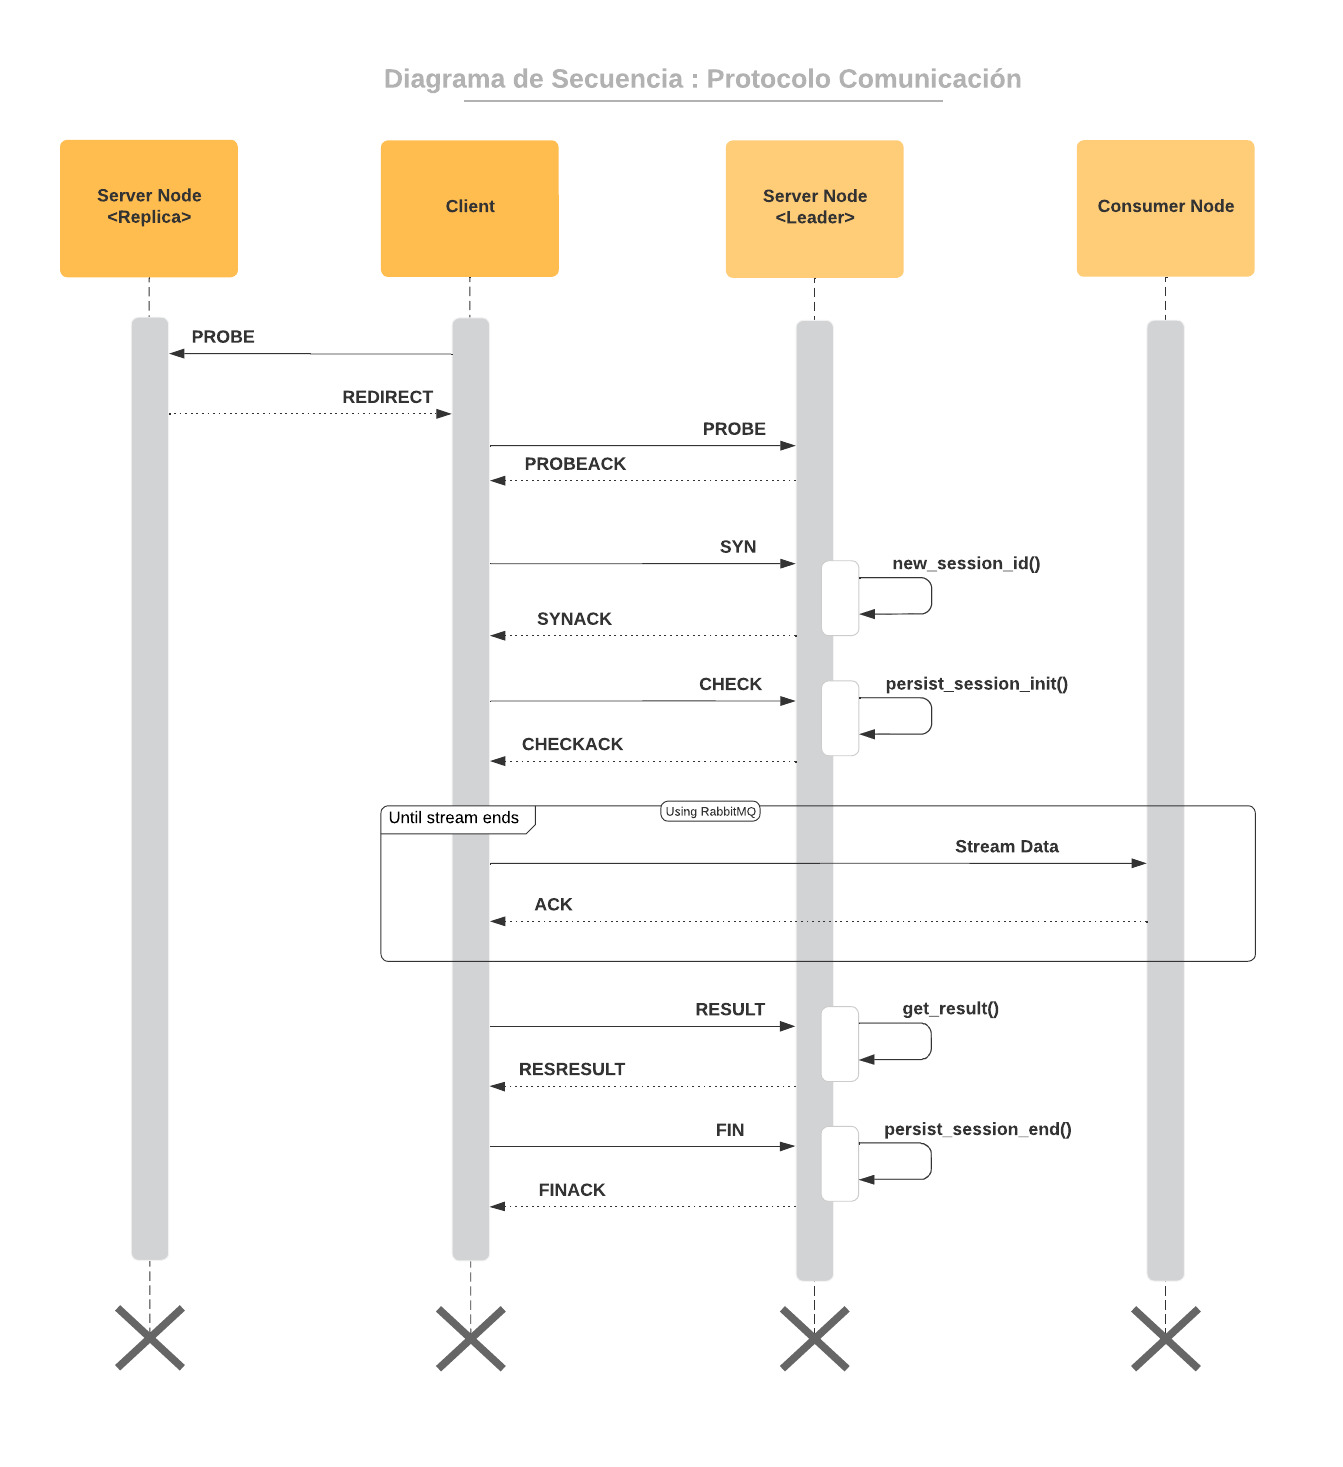
\includegraphics[width=13cm]{img/protocolo_secuencia.jpeg}
	\caption{Diagrama de secuencia para el protocolo}
\end{figure}

El cliente comienza enviando un paquete a una réplica al azar, que tiene como objetivo obtener el host del nodo líder. Con esa información, el cliente podrá enviar una nueva petición a dicho nodo buscando establecer una nueva sesión. El servidor responderá con un error si existe una sesión activa o, caso contrario, con un nuevo identificador de sesión.

Con este identificador el cliente envía un nuevo paquete solicitando confirmación. El servidor, al recibir este mensaje, deberá confirmar o negar la sesión al cliente. Si la sesión es rechazada, el cliente deberá reintentar este procedimiento nuevamente. En cambio, si la sesión es confirmada, el servidor responde con una serie de datos necesarios para que el cliente comience a enviar el stream. Justo antes del momento de confirmación el servidor deberá persistir la nueva sesión generada, para garantizar la existencia de la misma ante una caída.

A partir de este momento, cualquier comunicación con el servidor se realizará proveyendo el id de sesión en cada mensaje enviado.

En la respuesta del servidor se encuentra la información necesaria como para que el cliente se conecte a dos colas de RabbitMQ y comience a escribir el stream de datos sobre las mismas.

Una vez finalizado el envío del stream, el cliente procede a consultar periodicamente el resultado del cómputo al servidor. En cada consulta el servidor deberá preguntar por la existencia de resultados para dicha sesión a un nodo interno y responder con los mismos o con una negativa, en caso de haber sido completados.

Eventualmente, el cliente obtendrá los resultados y procederá a la fase de finalización de la sesión. En esta, el cliente envía un paquete de finalización y el servidor responde con una confirmación de la misma, dando lugar a un nuevo cliente. Nuevamente el servidor deberá persistir la finalización de la sesión del cliente antes de brindar una respuesta.

\paragraph{Tolerancia a Fallos}

Como ya se comentó, el servidor deberá almacenar el estado de la sesión del cliente actual. Para garantizar la existencia de la misma, aún ante escenarios de fallos, el servidor utiliza el protocolo de comunicación antes comentado, en combinación con un storage de datos distribuido entre los nodos que lo componen.

El nodo lider persiste el estado de la sesión en tres oportunidades distintas.

\begin{enumerate}
    \item Cuando se recibe un mensaje SYN conteniendo un id de sesión válido se persiste el estado de la nueva sesión y se confirma la misma al cliente.
    \item Cuando se recibe un resultado de computo del Collector, el mismo es persistido.
    \item Cuando el cliente decide dar por finalizada la sesión, el servidor persiste dicho estado, para dar lugar a un nuevo cliente.
\end{enumerate}

El diseño de este protocolo buscó lograr que ante cualquier fallo no se llegase a un estado incompatible como puede ser una sesión fantasma nunca reportada a un cliente o un desconocimiento de una sesión previamente iniciada por parte del servidor a un cliente.

\paragraph{Storage Distribuido}

El storage distribuido utilizado en el servidor se basa en la utilización de colas y exchanges del MOM.

Cada nodo del grupo servidor posee una cola persistente exclusiva a él que se encuentra bindeada a un exchange. Por dicho exchange el líder enviará cada actualización de las previamente comentadas. Dicha información será replicada y almacenada en cada una de las colas de los nodos, incluyendo la del propio líder.

Ante un cambio de líder, un reinicio del sistema, o una recuperación del mismo ante una caída, el storage entra en estado de recover. En dicho estado el proceso elegido como líder comienza a consumir su cola de datos hasta ponerse al día con el estado del servidor. Cada dato consumido será además almacenado en disco local para asegurar su persistencia.

El storage podrá garantizar que un nodo ha consumido todo el estado disponible con la utilización de un token. Antes de comenzar el proceso de recuperación, el storage envía un mensaje token por dicha cola que delimita el fin de los mensajes por consumir. Cuando dicho mensaje es consumido, se tiene garantía que el estado ha sido recuperado en su totalidad.

El siguiente diagrama busca representar dicha recuperación.

\begin{figure}[H]
	\centering
	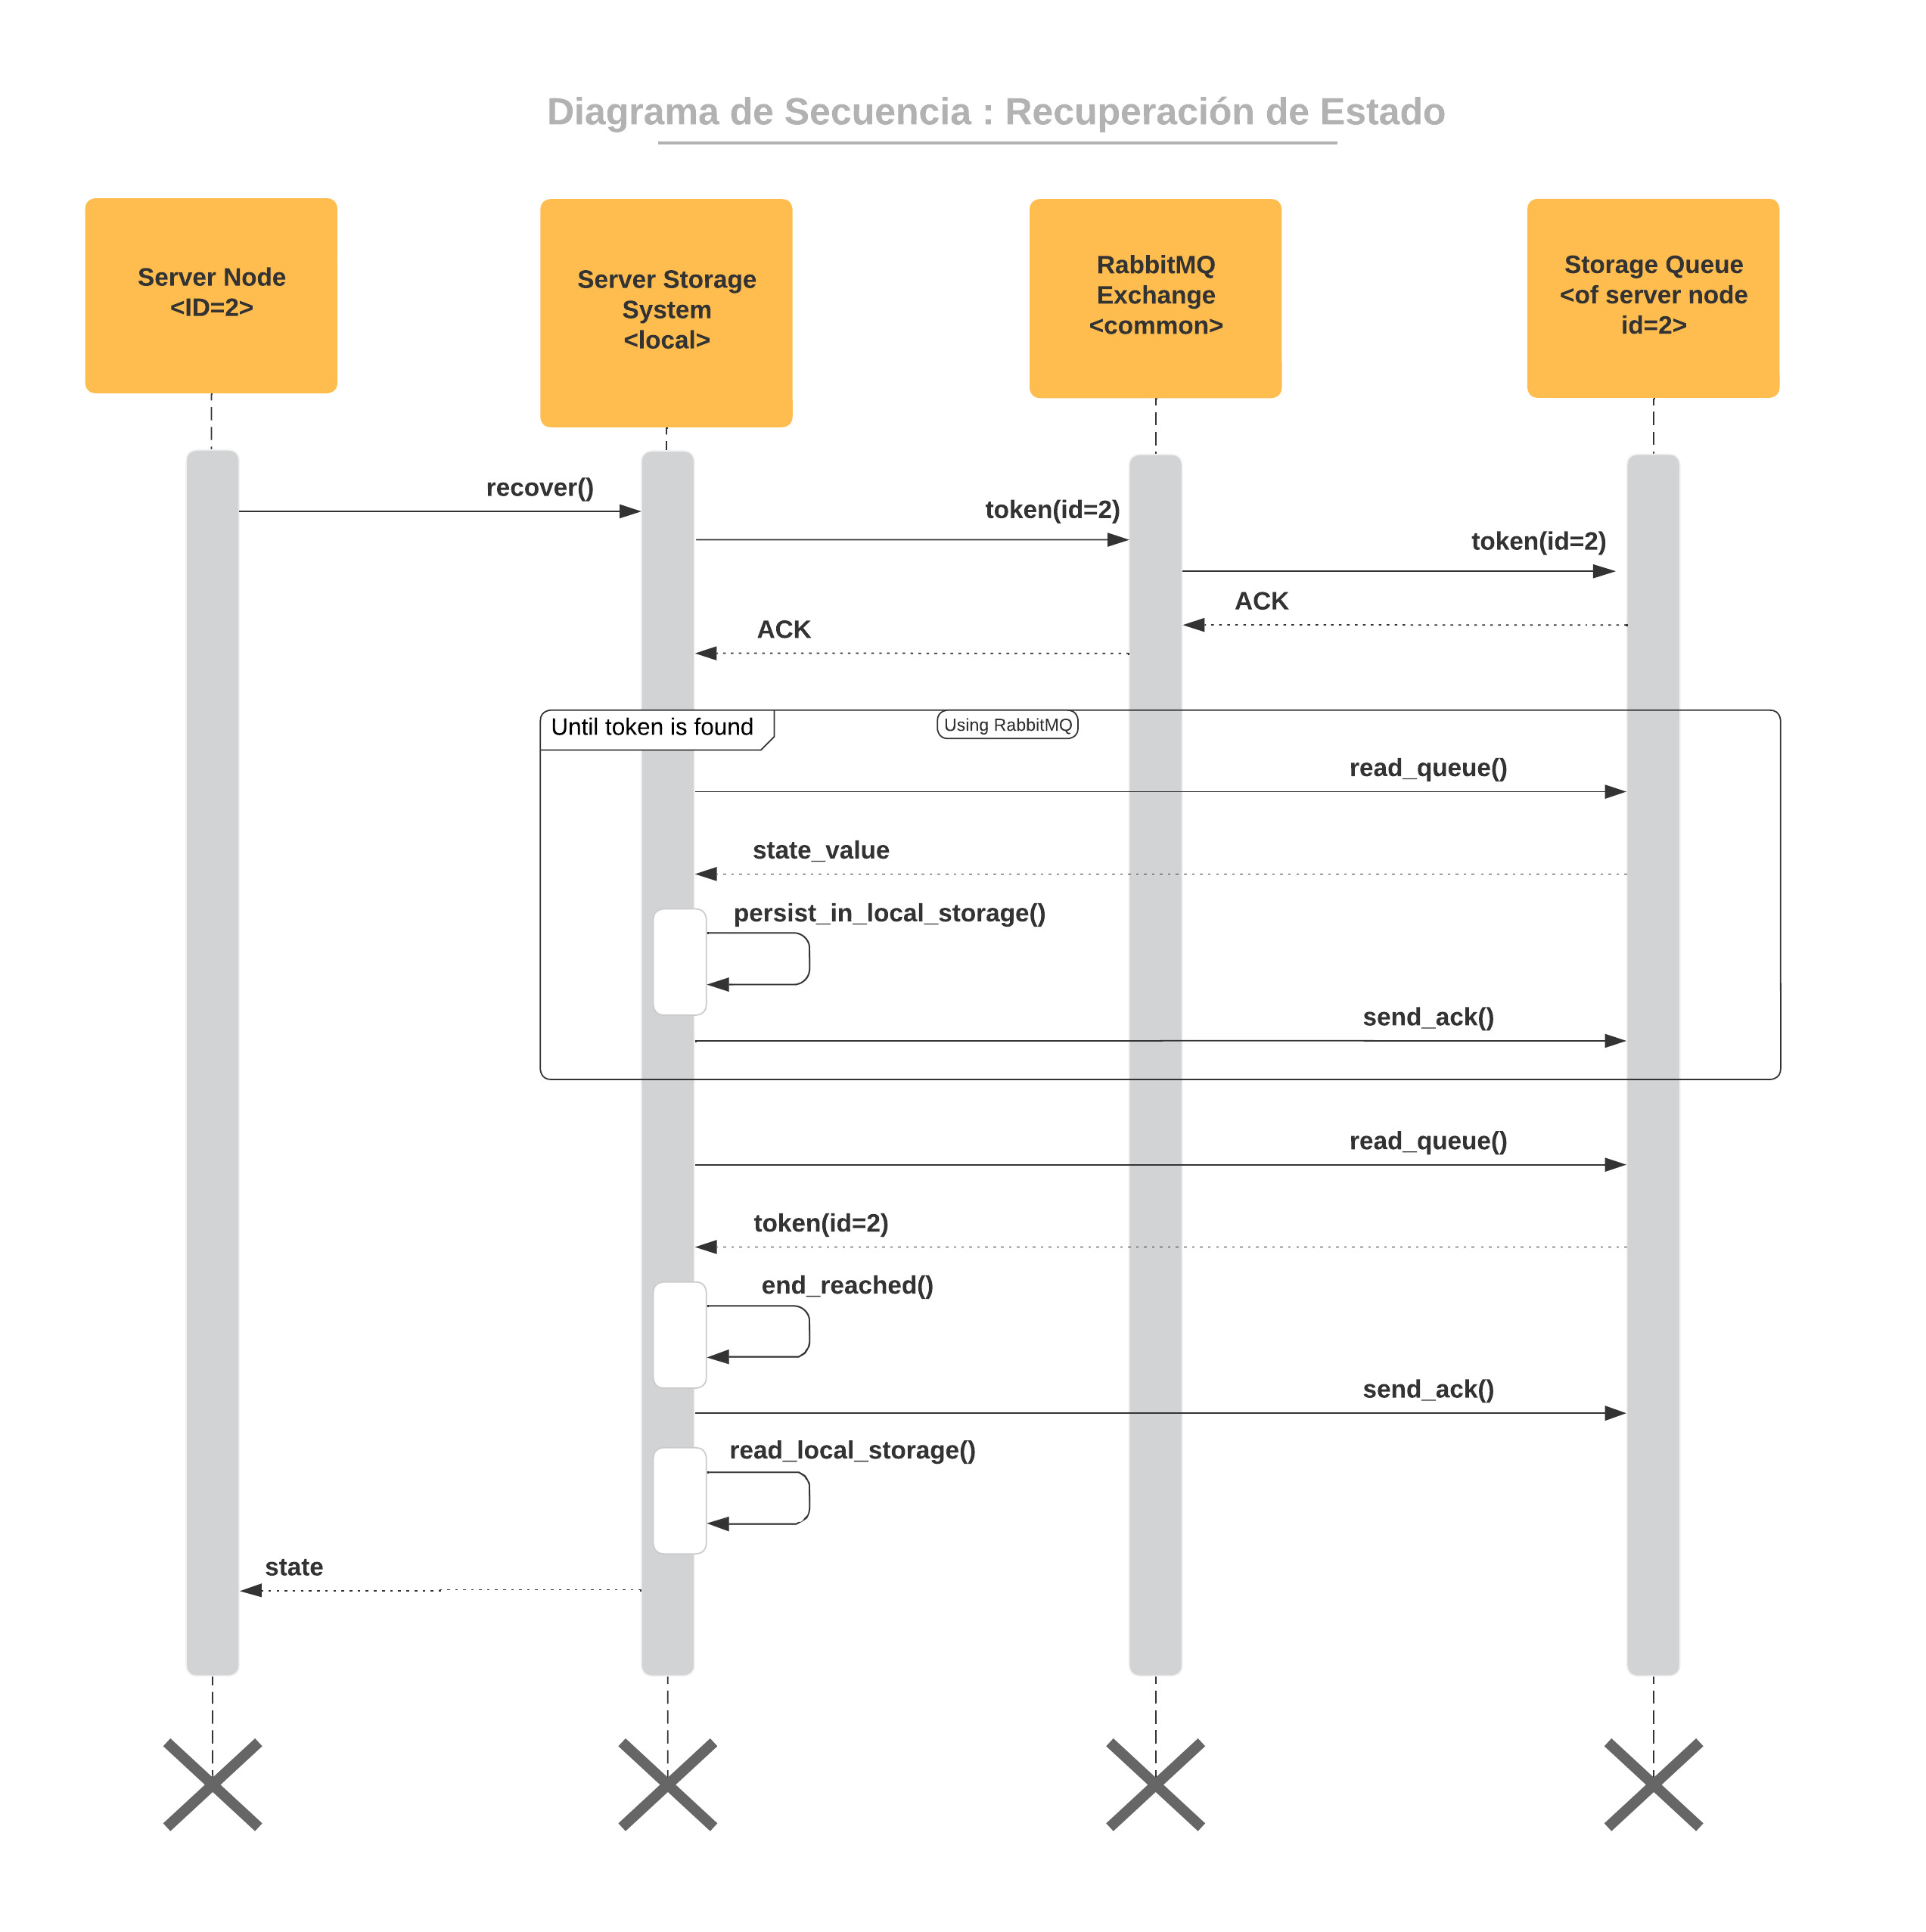
\includegraphics[width=13cm]{img/sequence_server_storage.jpeg}
	\caption{Diagrama de secuencia para el recover del server}
\end{figure}

Para poder cumplir este protocolo, el cliente debe tener una lista de preferencias de direcciones \texttt{host:port} de instancias de servidores de cara al cliente las que se pasan como variables de entorno o archivo de configuración, y deberá enviar el ACK al servidor una vez que haya pedido y obtenido exitosamente el resultado (el cual luego podrá tratarlo como sea que lo requiera).


\subsection{Coordinador}

Al comenzar se levanta el contenedor del coordinador quien es el encargado de observar el estado de todos los nodos del sistema y revivir aquellos que no responden. Para comenzar cada servicio utiliza \textit{Docker in Docker}.

Un comentario importante a realizar sobre el coordinador es que este no posee ni elección de líder ni replicación, haciéndolo un cuello de botella en el sistema en general, ya que de caerse, se frena todo el progreso de la sesión actual del cliente. En futuras iteraciones, de manera no tan compleja se puede imitar lo implementado en el server para poder lograr mitigar este punto de fallo.

\subsubsection{Heartbeats}

Cada nodo que deba ser monitoreado por el coordinador y revivido si se cayera, debe instanciar el \textit{sidecar} \texttt{HeartbeatSender} y ejecutarlo antes de su loop principal de ejecución.

Este \textit{sidecar} utiliza un socket \texttt{PUB} de \texttt{ZMQ} para enviar periódicamente un heartbeat que anuncia que está activo.

\subsubsection{Monitoreo de Heartbeats}

El Coordinador en lugar de instanciar el \textit{sidecar} \texttt{HeartbeatSender}, instancia el \textit{sidecar} \texttt{HeartbeatListener}. Este proceso levanta un hilo por cada contenedor al cual debe escuchar. Frente a una cantidad configurable de \textit{misses}, ejecuta un callback de error.

De este modo, al iniciar el sistema todos los nodos fallarán en sus heartbeats y el coordinador los revivirá: en su callback de error de heartbeats, revive al host que esté inactivo.

A fin de conocer todos los contenedores que debe monitorear y con que comandos revivirlos, el coordinador evalúa la configuración en uso, en principio leída de \texttt{settings.ini} y sobreescribible por variables de entorno.


\subsection{Despliegue del sistema}

\begin{figure}[H]
	\centering
	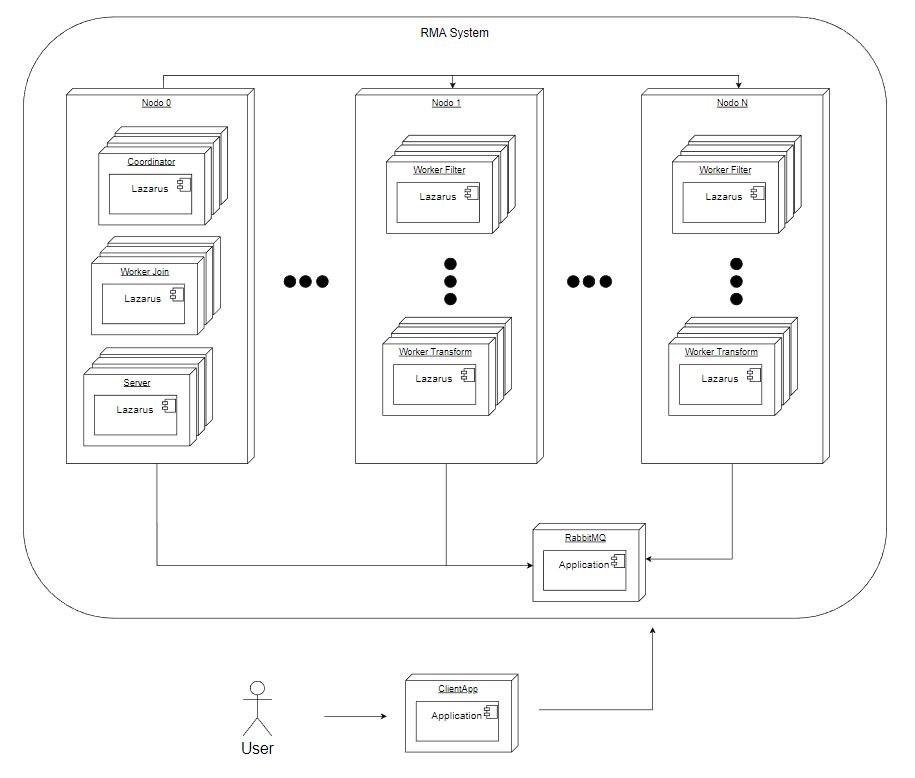
\includegraphics[width=13cm]{img/despliegue.JPG}
	\caption{Diagrama de despliegue}
\end{figure}

Como se observa, en principio cada proceso podría correr en una computadora distinta, por lo que se trata de un sistema multicomputing. Adicionalmente, las conexiones entre cada uno de los procesos se abstraen a través de la utilización de RabbitMQ como ya se comentó anteriormente, a excepción de las conexiones por ZMQ realizadas entre las réplicas del Servidor y el Coordinador con el resto de los procesos.


\section{Algoritmo de elección de líder}

El algoritmo de elección de líder implementado es \textit{bully}. De manera muy resumida, se basa en que en cualquier momento de la ejecución un nodo puede llamar a la elección de líder, la cual involucra un pasaje de mensajes por todos los nodos del grupo donde se hará la elección, hasta llegar a un consenso sobre cual será el nodo victorioso.

Este algoritmo se corre en un listener aparte, similar al que se tiene en el \textit{sidecar} para escuchar heartbeats, para que todo nodo pueda en cualquier momento responder un mensaje de elección (o de victoria).

La implementación debe:

\begin{itemize}
    \item Manejar correctamente el conflicto de dos nodos llamando a una elección de líder en simultáneo
    \item Proveer una interfaz para saber el estado de la ejecución (se esta decidiendo un líder, se tiene un líder conocido)
    \item Proveer una interfaz para saber el líder del grupo, y si yo soy el líder
\end{itemize}

\section{Almacenamiento}\label{APIStorage}
En esta primera versión del sistema desarrollado, se implementó una versión en almacenamiento local de una API genérica de persistencia de datos. Esta misma API podría implementarse como un sistema de archivos replicado entre nodos y ser reemplazado, creemos, de modo casi totalmente transparente.

Esta API introduce tres nociones:
\begin{itemize}
\item \textbf{Tópicos}: Son agrupaciones semánticas de pares clave-valor. Su uso es opcional, pero recomendado para separar datos de distintos contextos.
\item \textbf{Claves}: Son identificadores únicos dentro de un tópico (o dentro del tópico por defecto).
\item \textbf{Valores}: Los valores pueden ser cualquier objeto que pueda ser serializado a JSON.
\end{itemize}

La API de almacenamiento es la que permite validar si un mensaje ya ha sido visto anteriormente. Frente a un mismo mensaje, y asumiendo que la creación/obtención de su identificador es determinística, permite verificar eficientemente si ese identificador ya ha sido almacenado.

De modo de recuperarse frente a caídas, los objetos de almacenamiento deben tener afinidad con su carpeta de almacenamiento, la cual se define al momento de inicialización. Al crearse una nueva instancia, lee los archivos de su directorio de almacenamiento y reprocesa en orden los mensajes allí almacenados. Cada tópico se puede procesar independientemente, y es importante revisar que las líneas/archivos no estén corruptas. El primer caso se solucionó agregando un checksum a cada linea, de modo que si algún dato se ha corrompido, se detecte y descarte. Los archivos que respaldan los objetos de almacenamiento tienen formato \texttt{JSONL}\footnote{https://jsonlines.org}. Por tanto, las lineas corruptas mas allá de algunos simples caracteres, no podrían ser parseadas y descartadas. El caso de detección de archivos corruptos no fue atacado. Sin embargo, se plantea duplicar y rotar los archivos con cierta frecuencia, hacer copias de seguridad y solo agregar nuevos datos si se ha persistido correctamente el estado actual.

Los Nodos pueden hacer uso del \textit{modo de recuperación} al momento de empezar su ejecución. En este modo no permite escrituras/modificaciones. Iterando los tópicos donde hubiesen guardado mensajes, pueden emular su flujo original de manejo de mensajes, asegurándose de que no harán modificaciones/adiciones indeseadas al almacenamiento.

\printbibliography

\end{document}
